%=====================================================================
%  A1 PORTRAIT ACADEMIC POSTER
%  Surface-Code Syndrome Utilization for Fault Identification
%
%  Compile on Overleaf with pdfLaTeX (self-contained, no shell-escape).
%  Figures live in ./figures/ (real analysis outputs from the codebase).
%=====================================================================
\documentclass[17pt, a1paper, portrait, margin=0mm, innermargin=15mm,
               blockverticalspace=7mm, colspace=14mm, subcolspace=8mm]{tikzposter}

\usepackage[utf8]{inputenc}
\usepackage{lmodern}
\usepackage{amsmath, amssymb}
\usepackage{graphicx}
\usepackage{booktabs}
\usepackage{multicol}
\usepackage{tikz}
\usetikzlibrary{arrows.meta, positioning, shapes.geometric, backgrounds, fit}

%----------------------------------------------------------------------
% Colour palette
%----------------------------------------------------------------------
\definecolor{NavyDeep}{HTML}{0B2545}
\definecolor{Ocean}{HTML}{13476B}
\definecolor{Teal}{HTML}{1F8A8C}
\definecolor{Amber}{HTML}{E8A33D}
\definecolor{Coral}{HTML}{D64545}
\definecolor{Cloud}{HTML}{EEF3F7}
\definecolor{Ink}{HTML}{16222E}

%----------------------------------------------------------------------
% Theme
%----------------------------------------------------------------------
\usetheme{Default}
\usecolorstyle{Default}

\colorlet{backgroundcolor}{white}
\colorlet{framecolor}{NavyDeep}
\colorlet{titlefgcolor}{white}
\colorlet{titlebgcolor}{NavyDeep}
\colorlet{blocktitlebgcolor}{Ocean}
\colorlet{blocktitlefgcolor}{white}
\colorlet{blockbodybgcolor}{white}
\colorlet{blockbodyfgcolor}{Ink}
\colorlet{innerblocktitlebgcolor}{Cloud}
\colorlet{innerblocktitlefgcolor}{NavyDeep}

\settitle{
  \centering
  \vspace{3mm}
  {\color{titlefgcolor}\bfseries\Huge
   Surface-Code Syndrome Utilization for Fault Identification\par}
  \vspace{4mm}
  {\color{titlefgcolor}\Large
   Can repeated stabilizer syndromes reveal \emph{where} a device is faulty\,---\,not just \emph{that} it is?\par}
  \vspace{5mm}
  {\color{titlefgcolor}\large
   \textbf{Jaehun Han}\,$^{1}$ \quad
   \textit{[co-authors / advisor placeholder]}\,$^{1}$ \qquad
   $^{1}$[Institution / Group placeholder]\par}
  \vspace{2mm}
  {\color{titlefgcolor}\normalsize
   \texttt{pjhhan.research@gmail.com} \quad\textbullet\quad
   Niels Bohr Quantum Summer School 2026\par}
  \vspace{2mm}
}

%----------------------------------------------------------------------
% Handy macros
%----------------------------------------------------------------------
\newcommand{\keyfig}[3]{% file, width, caption
  \begin{center}
    \includegraphics[width=#2]{#1}\\[2mm]
    {\small\itshape #3}
  \end{center}}

\newcommand{\bignum}[2]{% number, label
  {\color{Coral}\bfseries #1}~{\small #2}}

% remove the default "LaTeX TikZposter" watermark
\tikzposterlatexaffectionproofoff

\begin{document}
\maketitle[titletotopverticalspace=5mm, titletoblockverticalspace=10mm]

%======================================================================
\begin{columns}
%==================== LEFT COLUMN =====================================
\column{0.5}

%---------------------------------------------------------------
\block{1.\ Motivation}{
\textbf{Surface codes already measure syndromes every round}\,---\,thousands of
stabilizer bits are produced purely to detect and decode errors, then discarded.

\vspace{2mm}
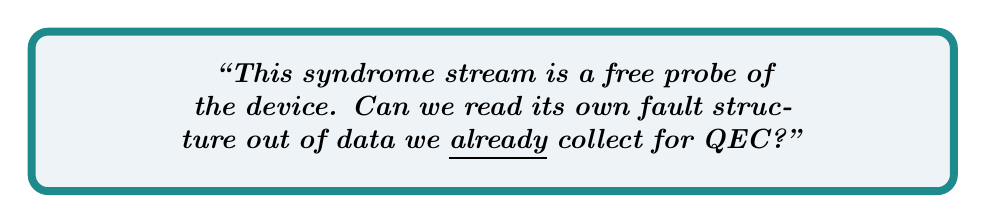
\begin{tikzpicture}
  \node[draw=Teal, line width=1mm, rounded corners=6pt, fill=Cloud,
        text width=0.9\linewidth, align=center, inner sep=4mm]
  {\bfseries
   \textit{``This syndrome stream is a free probe of the device. Can we read its
   own fault structure out of data we \underline{already} collect for QEC?''}};
\end{tikzpicture}

\vspace{3mm}
Long-term vision: a \textbf{closed loop} that recycles QEC data into device
knowledge, then feeds it back into better decoding.

\vspace{2mm}
\begin{center}
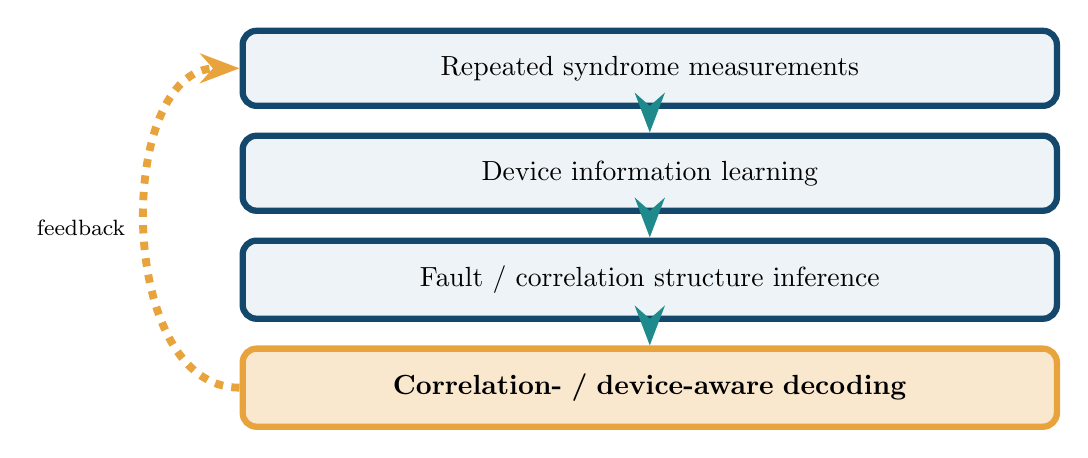
\begin{tikzpicture}[
  node distance=3mm,
  stage/.style={draw=Ocean, line width=0.8mm, rounded corners=5pt,
     fill=Cloud, text width=0.80\linewidth, align=center, inner sep=3.2mm},
  arr/.style={-{Stealth[length=5mm]}, line width=1mm, Teal}]
  \node[stage] (a) {Repeated syndrome measurements};
  \node[stage, below=of a] (b) {Device information learning};
  \node[stage, below=of b] (c) {Fault / correlation structure inference};
  \node[stage, below=of c, fill=Amber!25, draw=Amber] (d)
        {\textbf{Correlation- / device-aware decoding}};
  \draw[arr] (a) -- (b);
  \draw[arr] (b) -- (c);
  \draw[arr] (c) -- (d);
  \draw[arr, Amber, dashed] (d.west) to[out=180,in=180]
        node[left=1mm, font=\footnotesize, black]{feedback} (a.west);
\end{tikzpicture}
\end{center}

\vspace{1mm}
{\small This poster reports the \textbf{first link}: what fault information is\,---\,and
is \emph{not}\,---\,recoverable from syndromes alone.}
}

%---------------------------------------------------------------
\block{2.\ Case Study \& Problem}{
\textbf{Setting.} Distance-3 rotated surface code (17 qubits: 9 data + 8 ancilla);
each stabilizer-extraction round issues \textbf{24 directed CNOTs}. One CNOT is the
\emph{dominant} fault source (higher fault probability than the rest).

\vspace{2mm}
\begin{center}
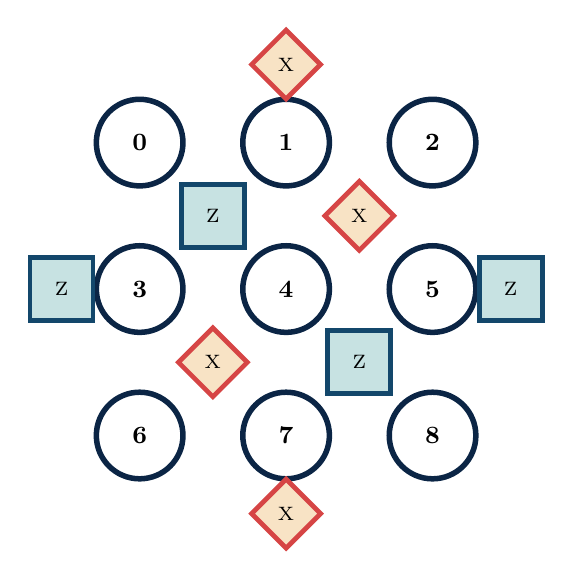
\begin{tikzpicture}[scale=0.62,
  data/.style={circle, draw=NavyDeep, line width=0.7mm, fill=white,
     minimum size=11mm, font=\small\bfseries},
  zanc/.style={rectangle, draw=Ocean, line width=0.6mm, fill=Teal!25,
     minimum size=8mm, font=\scriptsize},
  xanc/.style={diamond, draw=Coral, line width=0.6mm, fill=Amber!30,
     minimum size=9mm, font=\scriptsize}]
  \foreach \r in {0,1,2}{\foreach \c in {0,1,2}{
      \pgfmathtruncatemacro{\id}{\r*3+\c}
      \node[data] (d\id) at (\c*3.0, -\r*3.0) {\id};}}
  % interior weight-4 plaquettes (checkerboard)
  \node[zanc] at (1.5,-1.5) {Z}; \node[xanc] at (4.5,-1.5) {X};
  \node[xanc] at (1.5,-4.5) {X}; \node[zanc] at (4.5,-4.5) {Z};
  % boundary weight-2 stabilizers (outside the tile)
  \node[xanc] at (3.0, 1.6) {X}; \node[xanc] at (3.0,-7.6) {X};
  \node[zanc] at (-1.6,-3.0) {Z}; \node[zanc] at (7.6,-3.0) {Z};
\end{tikzpicture}\\[1mm]
{\footnotesize\itshape Rotated $d{=}3$ layout (schematic): data qubits (circles),
Z-/X-type ancillas (squares / diamonds).}
\end{center}

\vspace{2mm}
\innerblock{The question}{
From a temporal syndrome / detection-event sequence $S=(s_1,\dots,s_T)$
\emph{alone}, identify the \textbf{dominant faulty CNOT} among the 24.
\textbf{Nuisance factors} (unobserved): which rounds the fault fires, and its Pauli
type ($XX,\dots,ZZ$).}
}

%---------------------------------------------------------------
\block{3.\ Beyond Single-Shot}{
Exact enumeration (\S5) bounds \emph{single-shot} inference. Aggregating many noisy
sequences / shots can push past that ceiling.

\vspace{2mm}
\innerblock{Preliminary, naive $d{=}3$ model}{
Rule-based single-round \textbf{ceiling}: $18/24 = 0.75$. \\
Sequence model (GRU), temporal: \bignum{$\approx\!95\%$}{}. \\
Bag-of-shots (LogReg), spatial: \bignum{$\approx\!94\%$}{}.}

\vspace{2mm}
{\footnotesize Statistical aggregation breaks the rule-based ceiling\,---\,reported
as \textbf{preliminary}, not a final performance claim.}
}

%==================== RIGHT COLUMN ====================================
\column{0.5}

%---------------------------------------------------------------
\block{4.\ Temporal Information Threshold}{
Fix the Pauli type ($XZ$); enumerate the exact syndrome fingerprint of a single
fault at each CNOT and count how many of the 24 become distinguishable.

\vspace{2mm}
\keyfig{figures/fig_round1_degeneracy.png}{\linewidth}{%
  \textbf{One round.} Only \bignum{8}{of 24} CNOTs are uniquely identified;
  11 are syndrome-silent at round 0.}

\vspace{1mm}
\keyfig{figures/fig_round2_degeneracy.png}{0.82\linewidth}{%
  \textbf{Two rounds.} \bignum{24}{of 24} CNOTs uniquely identified\,---\,a sharp
  threshold; further rounds add no new information.}

\vspace{1mm}
\innerblock{Takeaway}{
With the Pauli type known, the \textbf{\emph{temporal} extent} of the record\,---\,not
its size\,---\,unlocks identification: $1\!\to\!2$ rounds moves $8/24\to24/24$.}
}

%---------------------------------------------------------------
\block{5.\ Cross-Pauli Ambiguity Wall}{
When the Pauli type is \emph{unknown}, distinct (CNOT, Pauli) faults can produce
\emph{identical} syndromes. Enumerating all $216$ cases:

\vspace{2mm}
\keyfig{figures/fig_collisions.png}{0.54\linewidth}{%
  Collision map: cell $(i,j)$ counts Pauli pairs making faults at CNOT$_i$ and
  CNOT$_j$ indistinguishable ($n_{\text{rounds}}{=}2$).}

\vspace{1mm}
\innerblock{Hard limit}{
The 216 cases collapse to 123 unique signatures with \bignum{72}{cross-CNOT
collisions}. With single-round faults and unknown Pauli type, \textbf{single-shot
24-class identification is information-theoretically impossible}\,---\,invariant
under round count and reset mode.}
}

\end{columns}

%==================== FULL-WIDTH FOOTER ===============================
\block{6.\ Status \& Outlook}{
\begin{minipage}[t]{0.32\linewidth}
  \textcolor{Teal}{\textbf{Done.}} Exact structural map of what syndromes
  can / cannot reveal about fault location at $d{=}3$.
\end{minipage}\hfill
\begin{minipage}[t]{0.32\linewidth}
  \textcolor{Amber}{\textbf{Ongoing.}} Stim-based \emph{realistic} circuit
  (parallel schedule, general $d$); \emph{probabilistic} dominant-fault model.
\end{minipage}\hfill
\begin{minipage}[t]{0.32\linewidth}
  \textcolor{Ocean}{\textbf{Next.}} Close the loop\,---\,feed inferred fault /
  correlation structure into \textbf{device-aware decoding}.
\end{minipage}

\vspace{4mm}
\begin{center}\small
Code, data \& figures: \texttt{Correlated-Noise-Estimation} repository
\quad\textbullet\quad Contact: \texttt{pjhhan.research@gmail.com}
\quad\textbullet\quad Niels Bohr Quantum Summer School 2026
\end{center}
}

\end{document}
